\section{Mini-Project B}
This project is for CS students only. Of course, if you'd like to attempt, you can.\\

\subsection{Scenario}
The biology student appreciates the work you have done developing a rough prototype. Their research has started gaining ground, and more people are becoming interested in their research. Because you did such a good job of developing the base system, the biology student has asked you to develop a means of a system where anyone can access their data. Being competent developers, well aware of web development, as well as being aware of the world of embedded systems you decide to use MQTT to transfer data. You want to make the system as accessible as possible, so you decide to use a low-cost Raspberry Pi to host a Node-Red server. For the sake of the prototype, you create a hotspot on the Raspberry Pi that people can connect to in order to access the server. You decide on the following design, as shown in Figure \ref{fig:NodeRed}:

\begin{figure}[H]
\centering
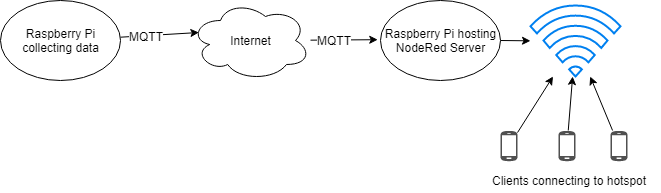
\includegraphics[width=0.8\columnwidth]{Figures/NodeRed}
\caption{Project B System Overview}
\label{fig:NodeRed}
\end{figure}

\subsubsection{Overview}
For this task, two Raspberry Pi's are required.One is to act as an MQTT broker, publishing the data gathered as per Mini Project A. The second is to act as an MQTT client that is subscribed to the first Pi and can be used to configure thresholds and display data using Node Red. A web page must be hosted on the second Pi, and it's WiFi interface should be turned into an access point. Devices should be able to connect to this access point, and view the web page.

Essentially, this is a repeat of the first project, but using a second Raspberry Pi with MQTT and Node Red as opposed to Blynk.

\subsubsection{Outcomes}
You will learn about:
\begin{itemize}
    \item MQTT (It's suggested you read \href{https://randomnerdtutorials.com/what-is-mqtt-and-how-it-works/}{this introduction to MQTT} and \href{https://cookbook.nodered.org/mqtt/}{MQTT on NodeRed}
    \item NodeRed (It's suggested you read \href{https://nodered.org/docs/getting-started/raspberrypi}{Getting Started with NodeRed on the RaspberryPi} to get started. There's also a nice plugin for good looking dashboards \href{https://flows.nodered.org/node/node-red-dashboard}{here}. You can also read the \href{https://learn.adafruit.com/raspberry-pi-hosting-node-red}{Adafruit Guide}.)
    \item Hosting an access point on the Pi. Notes are available in the lab handbook. 
\end{itemize}

\subsubsection{Deliverables}
At the end of this practical, you must
\begin{itemize}
    \item Demonstrate your implementation to a tutor. They will log in to your hotspot through their phone, view values, and adjust the alarm threshold.
    \item Submit a short write up. See the marking guide in section \ref{sec:ProjBMarks}
\end{itemize}

\subsubsection{Hardware Required}
You require the hardware from Project A, as well as a secondary Pi.

\subsubsection{Software Requirements}
\begin{itemize}
    \item You need to use an MQTT broker to publish and subscribe to messages relating to your practical. 
    \item You need to create a Node Red server that displays your data gathered from the first Raspberry Pi. 
    \item You will also need to have an option to adjust the alarm threshold from the NodeRed server.
\end{itemize}

\subsubsection{Marking Guide}
\label{sec:ProjBMarks}
\begin{table}[H]
\centering
\caption{The Write Up Format For mini-project B}
\label{tbl:ProjBMarks}
\begin{tabular}{|l|l|l|}
\hline
\textbf{Section of Report} & \textbf{Description} & \textbf{Marks} \\ \hline
\textbf{Introduction} & An introduction to what's new in this project & 10 \\ \hline
\textbf{Design} & \begin{tabular}[c]{@{}l@{}}Design of the system. Design of the server. \\ Talk about the stack used for development. \\ Include UML and block diagrams, and \\ mention any hardware/software\\ interfacing issues.\end{tabular} & 30 \\ \hline
\textbf{\begin{tabular}[c]{@{}l@{}}Implementation/\\ Build Proces\end{tabular}} & \begin{tabular}[c]{@{}l@{}}Some code snippets and steps in building \\ the device and server.Can think of this as a\\ simple methodology.\end{tabular} & 15 \\ \hline
\textbf{Instructions for use} & \begin{tabular}[c]{@{}l@{}}How to operate the system. You should \\ include some screenshots and photos.\end{tabular} & 15 \\ \hline
\textbf{Testing/Results} & \begin{tabular}[c]{@{}l@{}}How did you ensure your system works? \\ What did you do to test the functionality, \\ and what were the results? You can include\\ screenshots or photos, but you need to talk \\ about them (it's not enough to just have a \\ photo).\end{tabular} & 20 \\ \hline
\textbf{Conclusions} & \begin{tabular}[c]{@{}l@{}}How well did your system work? Did you \\ achieve the objectives? What could you do \\ to improve the system?\end{tabular} & 10 \\ \hline
\textbf{TOTAL} &  & \textbf{15} \\ \hline
\end{tabular}%
\end{table}

\subsubsection{Project B Validation Guide}
\label{sec:ProjBValidation}
\begin{table}[H]
\centering
\caption{Project B Demo Marks}
\label{tbl:ProjBValidation}
\resizebox{\textwidth}{!}{%
\begin{tabular}{|l|l|l|l|l|}
\hline
\multicolumn{2}{|l|}{\textbf{ProjB Validation Sheet}} & \multicolumn{3}{l|}{Marked By:} \\ \hline
\multicolumn{5}{|l|}{Student Numbers:} \\ \hline
\textbf{Component} & \textbf{Category} & \textbf{Description} & \textbf{Max marks} & \textbf{Mark} \\ \hline
\textbf{Hotspot} & Connectivity & \begin{tabular}[c]{@{}l@{}}Viewable in WiFi Menu \\ from phone\end{tabular} & 1 &  \\ \hline
 &  & Tutor can connect to it & 1 &  \\ \hline
\textbf{Node Red} & Implementation & WebPage is accessible & 1 &  \\ \hline
 &  & Starts on Boot & 1 &  \\ \hline
 & Design & \begin{tabular}[c]{@{}l@{}}All features of the\\ EnviroLogger should be\\ reflected in the webpage\\  (5 - LDR, pot, temp, \\ alarm, start/stop log)\end{tabular} & 5 &  \\ \hline
 &  & \begin{tabular}[c]{@{}l@{}}The use of widgets should \\ be aesthetically pleasing as \\ well as intuitive (use of labels, \\ placement of components)\end{tabular} & 3 &  \\ \hline
 &  & \begin{tabular}[c]{@{}l@{}}Can adjust the alarm \\ threshold (1) and is tested (2)\end{tabular} & 3 &  \\ \hline
\textbf{Marks Obtained} &  &  & \textbf{15} &  \\ \hline
\end{tabular}%
}
\end{table}
